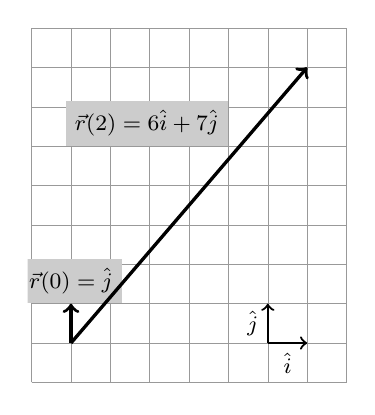
\begin{tikzpicture}[scale=0.5, help lines/.style={black!40,very thin}]
	\clip (-1.1,-1.1) rectangle (7.01,8.01);

	% Grid
	\draw[help lines] (-1,-1) grid +(8,9);

	% \vec r(0)
	\draw (0,1) node[anchor=south, fill=black!20!white] {\footnotesize $\vec r(0) = \hat j$};
	\draw[very thick] [->] (0,0) -- (0,1);

	% \vec r(2)
	\draw (4,5) node[anchor=south east, fill=black!20!white] {\footnotesize $\vec r(2) = 6\hat i + 7\hat j$};
	\draw[very thick] [->] (0,0) -- (6,7);

	% \hat i
	\draw[thick] [->] (5,0) -- ++(1,0);
	\draw (5.5,0) node[anchor=north] {\footnotesize $\hat i$};

	% \hat j
	\draw[thick] [->] (5,0) -- ++(0,1);
	\draw (5,0.5) node[anchor=east] {\footnotesize $\hat j$};
\end{tikzpicture}
